\documentclass[pdftex,12pt,a4paper,fleqn]{scrartcl}

\usepackage[utf8]{inputenc}
\usepackage[T1]{fontenc}

\usepackage[english]{babel}
\usepackage[babel]{csquotes}

\usepackage{lmodern}

\usepackage{microtype}

\usepackage{longtable}
\usepackage{array}
\def\arraystretch{1.5}

\usepackage{pdflscape}

\usepackage{amsmath}
\usepackage{amsfonts}
\usepackage{amssymb}

\usepackage[backend=biber,style=alphabetic]{biblatex}

\addbibresource{paper.bib}

\usepackage[paper=a4paper,margin=2.5cm]{geometry}

\clubpenalty = 10000
\widowpenalty = 10000
\displaywidowpenalty = 10000

\newcommand{\doctitle}{GPIO, I2C, and SPI on Embedded Devices}
\newcommand{\docauthor}{Maximilian Köhl}
\newcommand{\docemail}{mail@koehlma.de}
\newcommand{\docdate}{\today}

\usepackage[ngerman,pdfauthor={\docauthor},
            pdftitle={\doctitle},                 
            colorlinks=true,linkcolor=black,citecolor=black,urlcolor=black,
            filecolor=black]{hyperref}

\title{\doctitle}
\subtitle{\docsubtitle}
\author{\docauthor}
\date{\docdate}

\usepackage{setspace}

\usepackage[automark]{scrpage2}
\ihead[]{}
\ohead[]{}
\ifoot[]{\docauthor}
\cfoot[]{}
\ofoot[]{\thepage}
\pagestyle{scrheadings}

\usepackage[hang]{footmisc}
\setlength{\footnotemargin}{3mm}

\usepackage{todonotes}

\usepackage[framemethod=tikz]{mdframed}

\usepackage{graphicx}
\usepackage{subfig}

\usepackage{color}

\usepackage{float}

\usepackage{minted}

\parindent 0pt
\parskip 6pt

\begin{document}

\begin{titlepage}
	\begin{center}
		\vspace*{2cm}

		\vspace{4mm}
		{\Large\sffamily \textbf{\doctitle}} \\
		
		\vspace*{1cm}
		
		{\large \docauthor} \\
		\vspace{2mm}
		\docemail
		
		\vspace*{1cm}
		
		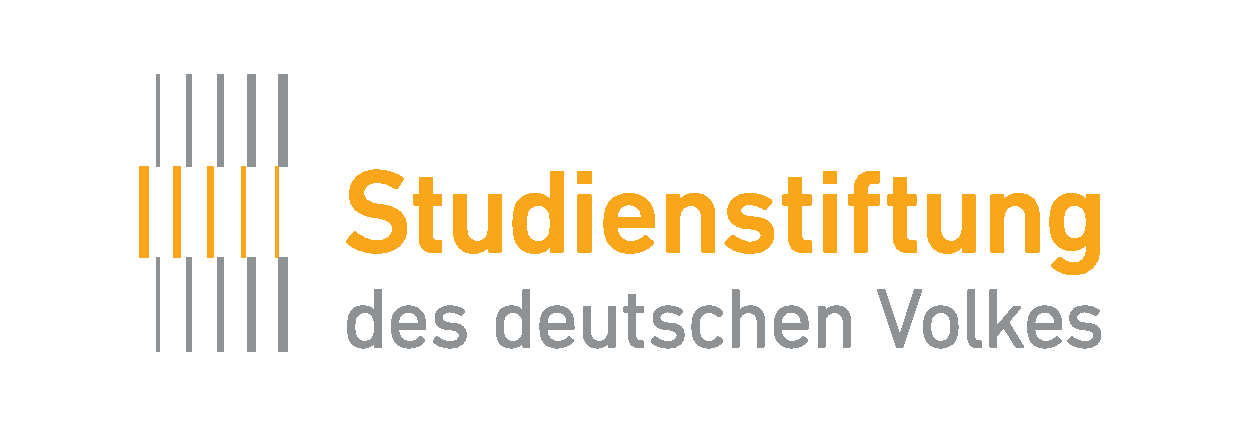
\includegraphics[width=8cm]{logo_sdv.pdf} \\
		{\large Sommerakademie in Leysin, August 2016}

	
	  \vspace*{1cm}
	
	  \begin{abstract}
	    \parindent 0pt
      \parskip 6pt
	    \noindent Embedded devices are already widely used in our every day lives without us noticing. With the internet of things they will no longer only control factories, mars rovers, waterworks but also our lights, doors, heating and air conditioning facilities, refrigerators and much more. Furthermore generic embedded platforms are affordable to everyone, not just large companies. Therefore it is possible for everyone to build their own embedded device.
      
      This paper aims to give you a brief overview about embedded and distributed systems as well as a compact introduction to GPIO and the two communication protocols I2C and SPI.
	  \end{abstract}
	
	  \vfill

	  \docdate
	\end{center}
\end{titlepage}

\newpage
\tableofcontents

\newpage

\section{Introduction}
This paper has been written in the context of the study group \enquote{Green Computing}\footnote{\url{https://greeniot.github.io/}} at the Sommerakademie of the Studienstiftung des deutschen Volkes in Leysin. It aims to cover two major topics in the field of embedded systems, namely the interaction with the physical environment and the communication with other embedded devices.

Because the focus of the study group was both theoretical and practical each topic will begin with an explanation of the theoretical foundations and finish with a closer look at practical applications of the theoretic aspects.


\section{Embedded Systems}
First of all I want to give you a short introduction to embedded systems and devices in general. Embedded devices are called embedded devices, because they are embedded into a larger system or product. Therefore they often need to interact with the physical environment or communicate with other embedded devices (figure \ref{fig:embedded_systems}).

\begin{figure}[H]	
	\centering
    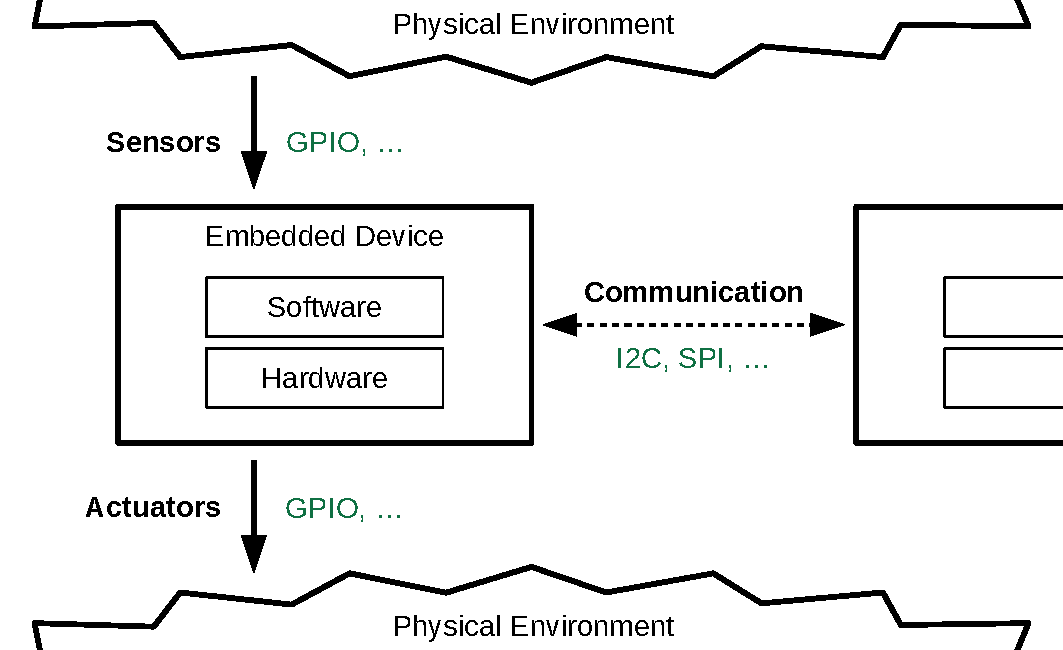
\includegraphics[width=.8\textwidth]{../Presentation/images/overview.pdf}
    \caption{Conceptual Schema of Embedded Systems}
    \label{fig:embedded_systems}
\end{figure}

To gather information about the physical environment an embedded device may be connected to several sensors. Basically there a two different kinds of sensors, analog and digital sensors. The former convert the physical value of interest into a voltage within a specific range whereas the latter encode the value into a digital signal. Digital means that there are only two possible values, logical high and low, corresponding to different voltage levels. In this paper we will focus on digital sensors. Digital sensors, for example a photo-transistor or a simple button, may be read out using GPIO.

In order to manipulate the physical environment an embedded device may be connected to several actuators. Again there are two different kinds of actuators, analog and digital actuators. The former take a voltage within a specific range whereas the latter are driven by a pure digital signal. In this paper we will focus on digital actuators. Digital actuators, for example a stepper-motor or a LED, may be driven using GPIO.

Since embedded devices may be connected to several sensors and actuators, they usually provide a bunch of different pins. For example the Arduino Uno (figure \ref{fig:arduino_uno}) provides 14 GPIO pins together with some special communication pins, but also pins for analog sensors or power supply pins for instance.

\begin{figure}[H]	
	\centering
    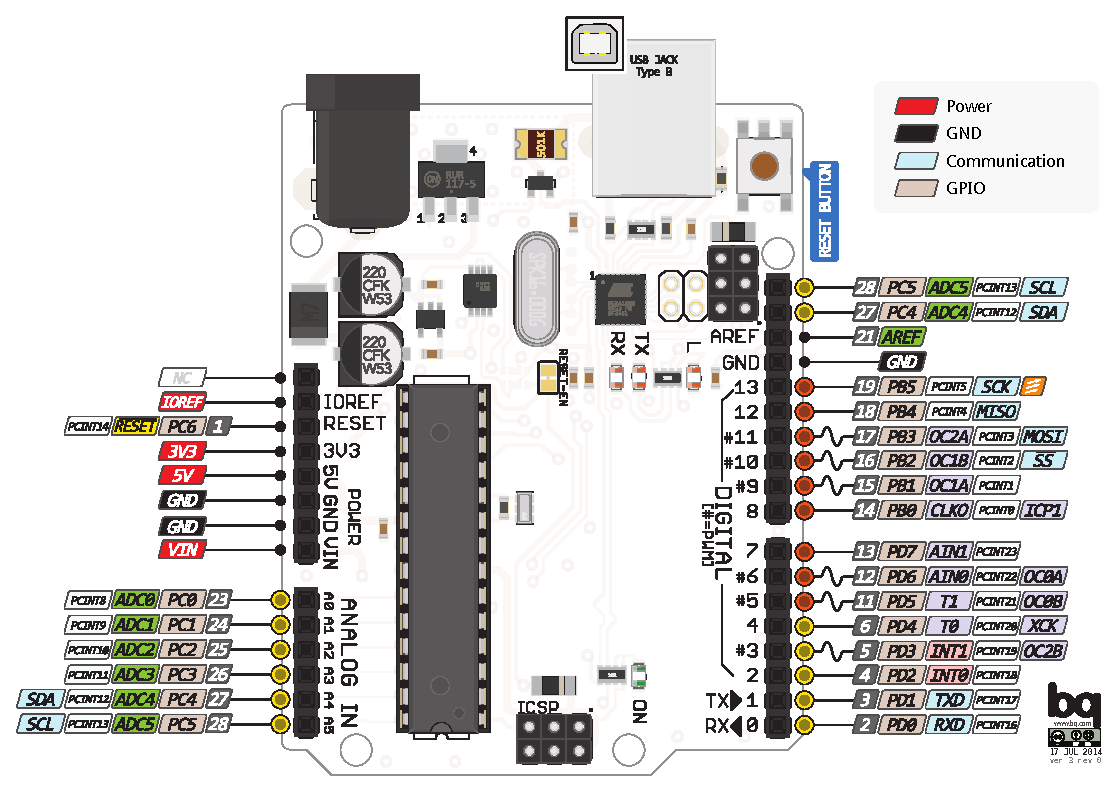
\includegraphics[width=.8\textwidth]{../Presentation/images/uno.pdf}
    \caption{Pins of the Arduino Uno}
    \label{fig:arduino_uno}
\end{figure}

Like every other computer system, embedded devices are discrete. However the real physical environment is not, it is continuous. Therefore when interacting with the physical environment or communicating with other embedded devices over some physical medium progress of time needs to be discretized. To discretize the time usually a square wave signal is used. Whenever this clock signal is logical high other signals must not change and the system is in a discrete state. When the clock signal is low other values might change until the next discrete step is indicated by a logical high clock signal.


\section{Input and Output}
Let us now go into more detail regarding the input and output capabilities of embedded devices and in particular the GPIO pins.

\subsection{GPIO}
GPIO stands for \enquote{General Purpose Input/Output} which means that the pin behavior is completely user specified and not predetermined by the manufacture of the device. GPIO pins are digital pins which means they can be in two different discrete states -- either logical high or low, corresponding to specific voltage levels.

As their name suggests, GPIO pins may be used in two different modes -- the input and the output mode -- which are selected by the software running on the device. When they are configured as an input, they are in high impedance state, which means they do not drain or provide any current. When they are configured as an output, they are in low impedance state, which means they drain or provide current.  To gather information from digital sensors the pin needs to be configured as an input and to drive digital actuators the pin needs to be configured as an output.

Some embedded devices also support interrupts on GPIO pins. An interrupt is a function which is called when for example the pin state changes from low to high. During the execution of the interrupt the main program is suspended.

In addition most embedded devices provide internal pull-up resistors which can be enabled by software. A pull-up resistor connects the pin with the logical high voltage level so the pin is in a well defined state if no other connection is present.

\subsection{Memory-Mapped IO}
Technically the input and output capabilities are usually implemented using memory-mapped IO. With memory-mapped IO there is, in addition to the classical ROM and RAM areas of the memory layout, a special area to talk to peripheral devices (figure \ref{fig:mmio_memory_layout}).

\begin{figure}[h]	
	\centering
    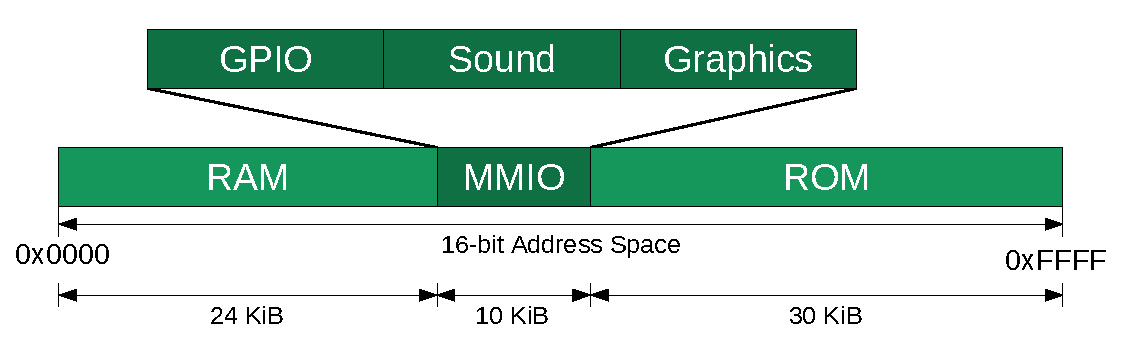
\includegraphics[width=.8\textwidth]{../Presentation/images/mmio.pdf}
    \caption{Typical Memory Layout}
    \label{fig:mmio_memory_layout}
\end{figure}

Peripheral devices are then simply used as if they were memory. The advantage of this approach is that only one bus is needed for both, memory and peripheral devices. For GPIO special bits at specific memory addresses indicate the configuration and status of each pin. When programming those devices in C the desired configuration of the GPIO pins is written directly to those addresses using pointers.

\subsection{Example: Arduino}
The programming language mainly used with the Arduino is some sort of special C++ but unlike normal C++ there is no explicit \mintinline{c}{main} function. Instead there are the two entry functions \mintinline{c}{setup} and \mintinline{c}{loop}. The former is executed once on startup and should contain all the initialization code, the latter is executed in a continuous loop and should contain the code for processing input and generating output.

The Arduino library provides low level primitives to directly interact with the GPIO pins. It implements three functions -- \mintinline{c}{pinMode}, \mintinline{c}{digitalRead}, and \mintinline{c}{digitalWrite}. To set the pin mode \mintinline{c}{pinMode} is used, which takes two arguments, the pin number and the mode which should be set. There are three different modes available, the output mode (\mintinline{c}{OUTPUT}), the input mode (\mintinline{c}{INPUT}), and the input mode with enabled pull-up resistor (\mintinline{c}{INPUT_PULLUP}). If a pin is configured to one of the input modes, \mintinline{c}{digitalRead} can be used to read out the state of the pin given the pin number. When configured as an output, \mintinline{c}{digitialWrite} can be used to set the state of the pin given the pin number and the logical state -- \mintinline{c}{HIGH} or \mintinline{c}{LOW} -- which should be written.

Enough theory – how does this look in practice? In the following I will demonstrate the usage of the GPIO pins of an Arduino with the Arduino library using the example circuit shown in figure \ref{fig:arduino_example}. We will implement a simple program which switches the LED off when the button is pressed and back on when it is released.

\begin{figure}[h]	
	\centering
  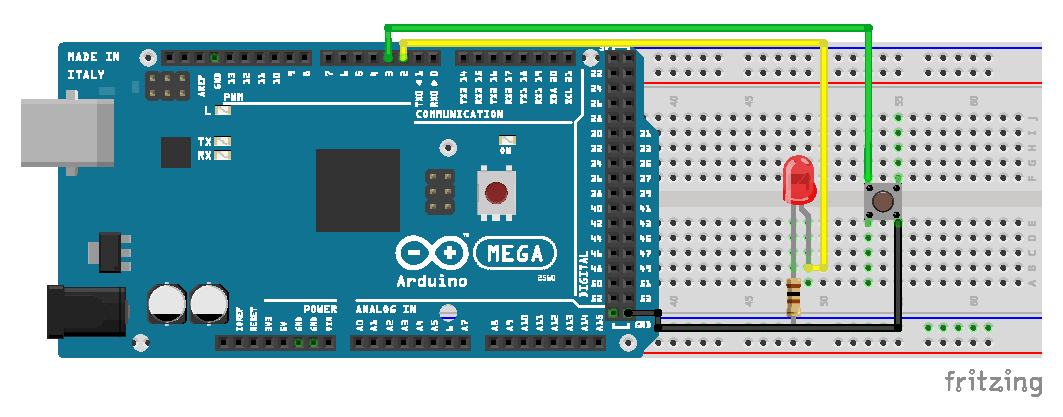
\includegraphics[width=.8\textwidth]{../Presentation/demo/circuit.pdf}
  \caption{Example Circuit using an Arduino}
  \label{fig:arduino_example}
\end{figure}

\begin{listing}[h]
\caption{Arduino Example Code}
\label{code:arduino}
\begin{minted}[linenos]{c}
#define BUTTON  3
#define LED     2

void setup() {
  pinMode(LED, OUTPUT);
  pinMode(BUTTON, INPUT_PULLUP);
}

void loop() {
  digitalWrite(LED, digitalRead(BUTTON));
}
\end{minted}
\end{listing}

The LED is connected to digital pin $2$ which therefore needs to be configured as an output. The button is connected with one side to ground and with the other to digital pin $3$ which therefore needs to be configured as an input with enabled pull-up resistor. This configuration takes place in the \mintinline{c}{setup} function. When the button is released, the pin is disconnected and becomes logical high because the pull-up resistor is pulling the pin to logical high voltage. When the button is pressed, the pin is connected to ground and therefore becomes logical low. Because of this somehow \enquote{inverted} behavior it suffices to continously write the state of the button pin directly to the LED pin to archive the behavior specified above. Listing \ref{code:arduino} implements the whole program.

\subsection{Example: Raspberry}
The well-known Raspberry Pi single-board computer provides GPIO pins as well. Again they are accessible using low level primitives. However because the Raspberry provides more computation power there are many high level libraries available for many different programming languages. The Johnny-Five\footnote{\url{http://johnny-five.io/}} library for Node.js (JavaScript) which we are going to use in the following is one of them.

The code in listing \ref{code:raspberry} mimics the behavior of the Arduino code example. However it uses high level objects like \mintinline{javascript}{Led} and \mintinline{javascript}{Button}. The Johnny-Five library also provides events like \mintinline{javascript}{ready}, \mintinline{javascript}{up}, and \mintinline{javascript}{down} to simplify programming. I do not want to go into much detail here, if you are familiar with programming this example should be easily understandable.

\begin{listing}[H]
\caption{Raspberry Example Code}
\label{code:raspberry}
\begin{minted}[linenos]{javascript}
var raspi = require('raspi-io');
var five = require('johnny-five');
var board = new five.Board({ io: new raspi() });
      
board.on("ready", function() {
  var led = new five.Led("P1-2");
  var button = new five.Button("P1-3");
        
  led.on();
        
  button.on("up", function () {
    led.on();
  });
  button.on("down", function () {
    led.off();
  });
});
\end{minted}
\end{listing}


\section{Distributed Systems}
Nowadays most embedded systems are implemented in a distributed fashion which means that the system is split up into several components, called nodes. To deliver a specific service these components then communicate with each other over some realtime communication system (figure \ref{fig:distsys}). In contrast to a monolithic system a distributed design allows a modular system development. Components can be individually developed, tested and verified. In case of failure components can be replaced individually which also keeps repairing costs low. In safety critical systems introducing componentwise redundancy may also increase the overall reliability of the system. However these advantages come at the expense of needing a reliable realtime communication system. In this section we are focusing on different approaches to communication systems. The most important question is probably, how do the nodes communicate? Here a communication protocol comes into play.

\begin{figure}[h]	
	\centering
  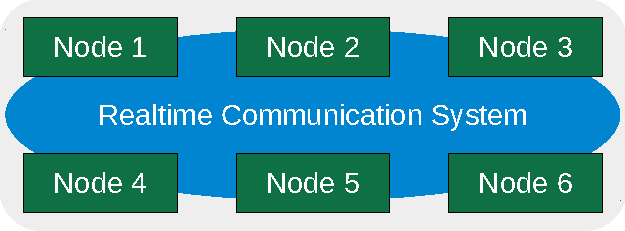
\includegraphics[width=.45\textwidth]{../Presentation/images/node-com.pdf}
  \caption{Conceptual Scheme of a Distributed System}
  \label{fig:distsys}
\end{figure}

\subsection{Communication Protocols}
A communication protocol is simply a contract about how to communicate. Some communication protocols only specify how things look like on the data layer, others also include specification for connectors and the physical layer. Basically there a two different types of protocols, stream and message based protocols. Stream based protocols deliver a constant data stream whereas massage based protocols deliver discrete entities of information called a message. We are focusing on message based protocols in this paper.

We distinguish two different kinds of messages, event messages and state messages. Event messages carry information about a particular event, for instance \enquote{The button has been pressed!} whereas state messages carry state information, for instance \enquote{The button is pressed!}. These message kinds play well together with different so called control strategies. A control strategy specifies when messages are sent. First of all there is the external control strategy where the decision is done by the software running on the node. Together with event messages this results in an event-triggered communication with explicit send commands and interrupts on message reception. On the contrary there is the autonomous control strategy where the decision is done by the communication system itself. Together with state messages this results in time-triggered communication where state information is exchanged on a regularly basis without interfering with the host computer. Both strategies have their own advantages and disadvantages.

\subsubsection{Requirements}
Communication protocols in embedded systems usually need to satisfy certain application specific requirements. In the following I want to give you an overview over some comon requirements without any claim to be comprehensive.

For many applications communication protocols need to meet safety critical realtime constraints. For example the break-by-wire system in a car has to guarantee that the breaks are reacting within a fixed time interval. 

In general communication protocols have to provide an appropriate bandwidth and communication delay but at the same time be cost and energy efficient.

If failures occur a communication protocol has to reasonable handle them without crashing the whole system, it should be robust and fault tolerant. Such that an error in the multimedia system of your car does not influence  any other vital car system.

Maintainability and diagnosability also became very important aspects of communication protocols and systems. Faults might be masked because of the fault tolerance mechanisms. Therefore these systems have to provide diagnosis and maintenance capabilities.

\subsubsection{Error Detection}
To provide fault tolerance error detection has to be done. Basically there a two different types of errors, transmission errors and node errors. Transmission errors are errors in the transmission of a message, for example bit flips or completely lost messages. To detect those errors a protocol might use checksums, which are mathematical functions computed over the message. The result of the function is transmitted together with the message such that the recipient can verify the integrity of the message by recalculating the checksum on its own and then compare those two. Some of these checksum mechanisms also allow the reconstruction of the original message if only some data has been corrupted.

Recipients may also send explicit acknowledgments such that the sender knows that the message has been successfully delivered. This way completely lost messages can be detected as well as node errors and the sender is able to react appropriately.

\subsubsection{Properties}
If we want to reason about communication protocols we first have to understand some key properties each communication protocol has. This section aims to give you a brief overview over the most important properties of communication protocols.

\paragraph{Latency and Jitter} Latency is the time a message takes in the communication system from being sent until it is delivered. Jitter is the variation in latency. Usually one aims for small latency which enables rapid communication with low distribution overhead. Also low jitter is wanted to ensure reliable temporal properties of messages.

\paragraph{Full- and Half-Duplex Communication} Full duplex communication protocols allow a simultaneous data flow in both directions at the same time. So while a node receives data is is at the same instant able to send data on its own over the system. Half duplex protocols on the contrary allow only unidirectional communication at every instant.

\paragraph{Flow Control} There is an inherent asymmetry between the sender and the recipient regrading the pace of data transmission. A sender might send data too rapidly for the recipient to handle. Therefore some flow control mechanism has to be established. There are two types of flow control, implicit flow control and explicit flow control. The former happens at design time by specifying the maximum pace all nodes need to be able to handle. So the pace is pre-determined by contract. The latter is done at run-time using explicit messages or other signals to control the transmission speed. So the receiver controls the pace explicitly by using those mechanisms.

\subsection{Network Topologies}
One important question has been left open until now: How to physically connect the nodes? There are several node connection schemes called network typologies. The most naive one would be to simply connect each node with all the other nodes. This topology is called the P2P topology (figure \ref{fig:p2p}). Because the number of necessary connections grows rapidly ($\mathcal{O}(n^2)$) this network topology is impractical for large networks. An other topology frequently used in embedded systems is the bus topology (figure \ref{fig:bus}) where all nodes are connected to a single communication bus.

\begin{figure}[H]
  \subfloat[P2P Topology]{%
    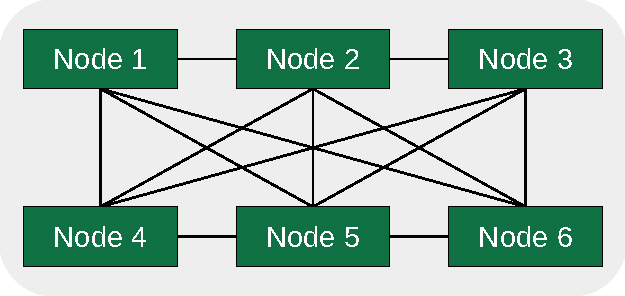
\includegraphics[width=.45\textwidth]{../Presentation/images/p2p.pdf}
    \label{fig:p2p}
  }
  \hspace{.8cm}
  \subfloat[Bus Topology]{%
    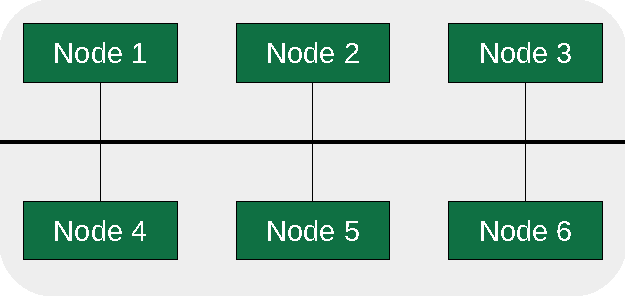
\includegraphics[width=.45\textwidth]{../Presentation/images/bus.pdf}
    \label{fig:bus}
  }
  \caption{Network Topologies}
\end{figure}

Compared to the P2P topology the bus topology is much more efficient in economic terms, because the reduced number and length of cables. The bus topology is also more modular, because a new node only has to be connected to the one central bus. This allows modular system development, support and evolution which was one of the key advantages of distributed systems in the first place. Recalling the requirements for a good communication protocol diagnosability is also very important. The bus topology allows efficient diagnosis by bus snooping. A debugging device may simply be connected to the bus and can than be used to sniff the whole bus traffic or for communication with a specific node. Because of all these advantages there has been a significant shift to bus typologies in the field of embedded systems. However the downside of this approach is that there needs to be some sort of bus access coordination.

\subsection{Bus Arbitration}
This access coordination is called bus arbitration. There are several approaches to solve this coordination problem. In general there is fundamental tension between small latency for important nodes/messages and sufficient as well as consistent service for less important nodes/messages. In practice there is an inverse relation between volume and urgency of a message. In the following I want to present to you three different approaches to bus access coordination -- time division multiplexed access, the bus master approach to coordination, and carrier sense multiple access.

\subsubsection{TDMA -- Time Division Multiplexed Access}
With the TDMA approach all nodes first have to agree on some global notion of time. After that the progress of time is divided into TDMA rounds. Within each round each node has a private time slot where only this node is allowed to send data – so the time slots have to be none overlapping (figure \ref{fig:tdma}).
 
\begin{figure}[h]	
	\centering
  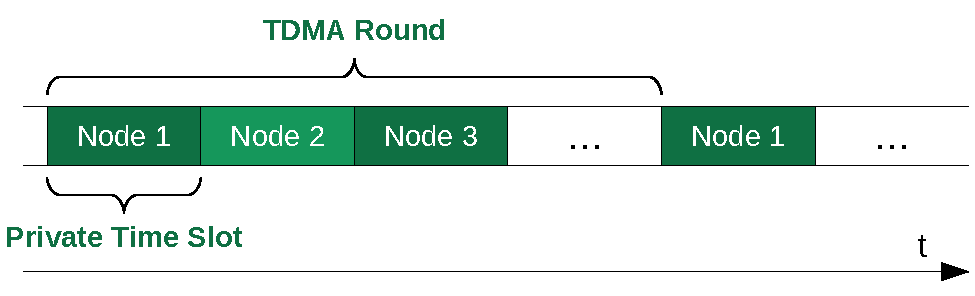
\includegraphics[width=.7\textwidth]{../Presentation/images/tdma.pdf}
  \caption{TDMA -- Time Division Multiplexed Access}
  \label{fig:tdma}
\end{figure}

Using the TDMA approach we get a guaranteed worst-case latency given by the period of the TDMA rounds. However the private time slots waste a lot of bandwidth if a node does not want to transmit any data. Also the number of nodes has to be fixed during the installation which limits the modularity of this approach.

\subsubsection{Bus Master Approach to Coordination}
The bus master approach to coordination is very simplistic. There are two different roles a node may have – the master role and the slave role. Only one master node is allowed on the bus (figure \ref{fig:bus_master_approach}). The master node is the only node allowed to access the bus on its own. All other nodes are slave nodes and are only allowed to write to the bus if the master granted permission to do so.

\begin{figure}[h]	
	\centering
  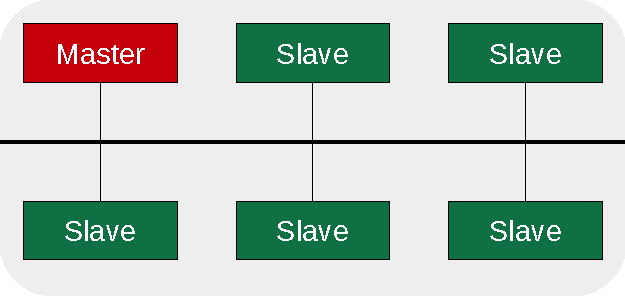
\includegraphics[width=.45\textwidth]{../Presentation/images/bus-master.pdf}
  \caption{Bus Master Approach to Coordination}
  \label{fig:bus_master_approach}
\end{figure}

To provide fault tolerance the systems has to deal with two different errors. First of all a slave node might be unresponsive or at least too slow. The master node may use timeouts to detect and counter such an error. The more problematic error is a faulty master node. To detect and counter this error a master node may send special heartbeat messages regularly. If a heartbeat is missing every node on the bus knows that there is something wrong with the master. The master may than be dynamically replaced by a spare node or after additional coordination by one of the previous slave nodes.

If a slave node wants to transmit some data it has to wait until the master granted permission to access the bus. Therefore the master needs to regularly poll a willing-to-send slave. Potential recipients simply listen to the bus traffic.

The major advantage of the bus master approach to coordination is its simplicity. Also the latency is bounded if the massage length is constrained. However the centralized master introduces a single point of failure and the polling consumes a lot of bandwidth. Also the number of nodes has to be fixed during the installation because the master needs to know which nodes to poll. Nevertheless the bus master approach is frequently used because it is very simple to implement.

\subsubsection{CSMA -- Carrier Sense Multiple Access}
With the CSMA approach there is a simple rule: A node is allowed to access the communication medium if it is idle. However two nodes might start sending a message almost simultaneously, which then leads to crippled or overwritten messages. To counter this a protocol have to provide some sort of collision detection. With the CSMA with collision detection (CSMA/CD) approach a node will back up if a collision has happened and waits for a random time until it tries to send the message again. An even more sophisticated approach is CSMA with collision resolution (CSMA/CR). With CSMA/CR collisions are resolved by the bus arbitration such that at least one message is delivered successfully. Later we will have a look at an example on how this could be implemented.

\subsection{Implementation}
Let's look at the actual implementation of communication protocols in embedded devices. Usually a node is split up into three different parts (figure \ref{fig:node_structure}). The communication controller handles all the lower level details of the communication protocol and provides a well defined interface, the communication network interface (CNI). The host computer, where a specific program is running then uses the CNI to access the communication medium.

\begin{figure}[h]	
	\centering
  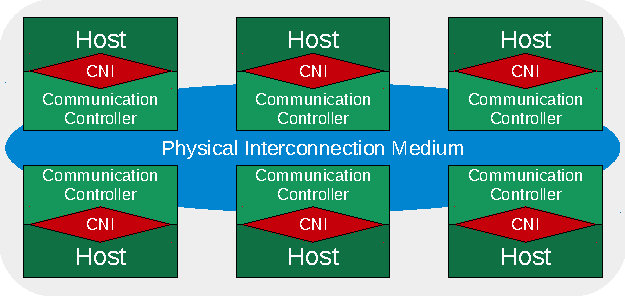
\includegraphics[width=.6\textwidth]{../Presentation/images/host-cni.pdf}
  \caption{Internal Node Structure}
  \label{fig:node_structure}
\end{figure}

Most modern micro controllers provide a variety of special purpose pins for various communication protocols together with a communication controller. For instance the Arduino Uno offers special purpose pins for the two protocols I2C and SPI (see figure \ref{fig:arduino_uno}). In the following two sections I will explain those protocols in more detail.

\subsection{I2C -- Inter Integrated Circuit [Protocol]}
Inter integrated circuit protocol (I2C) is a bus protocol using two signal wires – one wire for the digital clock (SCL) and one for the data (SDL). Both signal lines are pulled up using pull-up resistors which is crucial for the bus access coordination (see figure \ref{fig:i2c_physical}). 

\begin{figure}[h]	
	\centering
  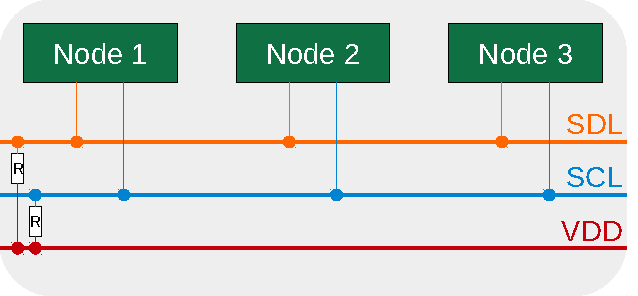
\includegraphics[width=.5\textwidth]{../Presentation/images/i2c-bus.pdf}
  \caption{I2C Physical Connection Scheme}
  \label{fig:i2c_physical}
\end{figure}

I2C uses the CSMA/CR approach to bus coordination. Therefore, if a node wants to send a message, it first has to wait until the bus is idle. When the bus is idle it starts by sending a start condition by pulling the SDL line low. Now other nodes know that there is a transmission ongoing, so the bus is blocked and the transmitting node starts generating a clock signal on SCL. The message is then written bit per bit on the SDL line. The bits are sampled during the clock signal is high. After transmitting the whole message the node first stops generating the clock signal and sends a stop condition (figure \ref{fig:i2c_timing}).

\begin{figure}[H]	
	\centering
  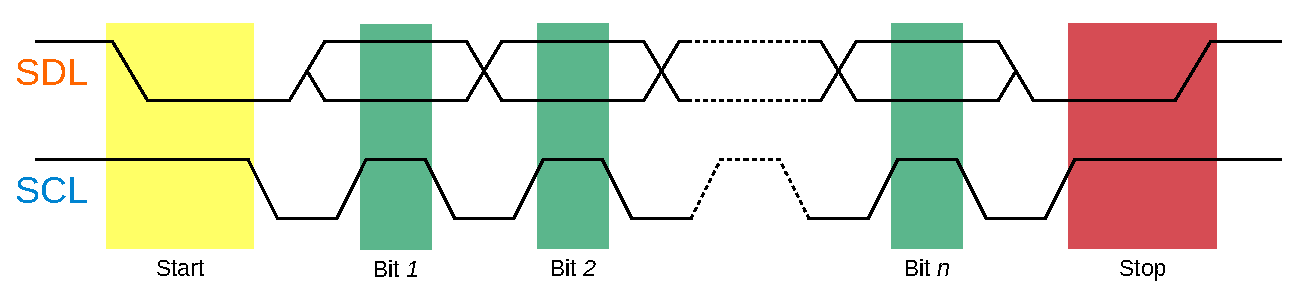
\includegraphics[width=.8\textwidth]{../Presentation/images/i2c-timing.pdf}
  \caption{I2C Timing Diagram}
  \label{fig:i2c_timing}
\end{figure}

A node might be either a master or a slave node. However the roles are only fixed for one message. The master nodes initiates the transmission and generates the clock signal whereas the slave node responds when being addressed. So each node which may act as a slave node has its own unique address. Addresses are $7$-bit wide which limits the number of slave nodes on the bus to $127$. The protocol specification specifies not only how bits are transmitted on the physical layer, but also which format messages should have (figure \ref{fig:i2c_msg}).

\begin{figure}[h]	
	\centering
  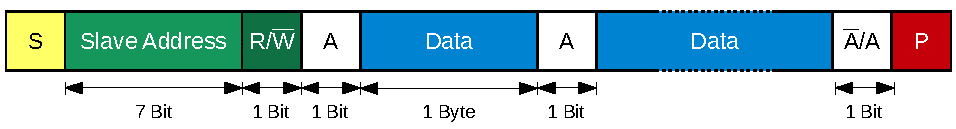
\includegraphics[width=.9\textwidth]{../Presentation/images/i2c-message.pdf}
  \caption{I2C Message Format}
  \label{fig:i2c_msg}
\end{figure}

A message starts with the start condition followed by the slave address the master wants to talk to. The last bit of the first byte specifics whether the master wants to read ($1$) or write ($0$) data. After the address and direction bit the slave sends an acknowledgment bit indicating it is ready to read or write data. If the master wants to read data the slave starts transmitting data byte per byte. Each byte is acknowledged by the master if it wants to receive more data. If the master does not want more data it does not acknowledge and stops the communication after that. If the master wants to write it starts sending data byte per byte. Each byte has to be acknowledged by the slave. If all data has been sent the master stops the communication. I2C also includes an explicit flow control feature. When the master sends too rapidly the slave may hold the clock line low until it is again able to handle more data. This mechanism is called clock stretching.

Because I2C supports multiple masters there have to be some sort of collision handling. I2C uses the CSMA/CR approach with bit arbitration. Because of the physical setup with the pull-up resistors low signal overwrite high signals.

\begin{figure}[H]	
	\centering
  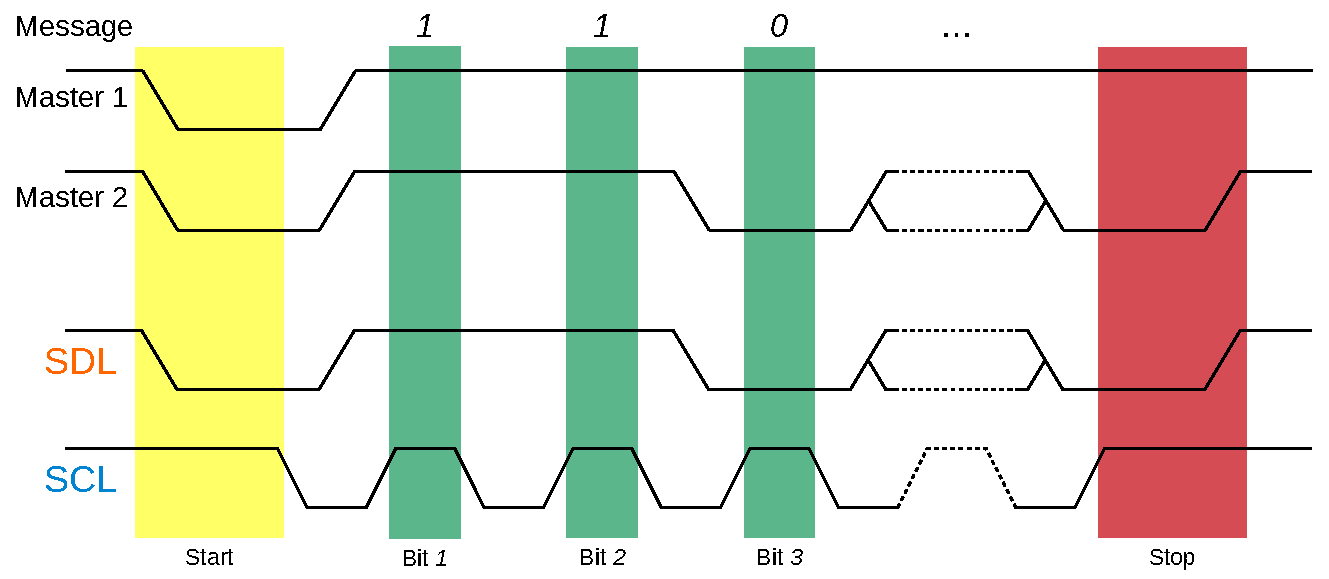
\includegraphics[width=.8\textwidth]{../Presentation/images/i2c-collision.pdf}
  \caption{I2C Timing Diagram with Collision}
  \label{fig:i2c_collision}
\end{figure}

Figure \ref{fig:i2c_collision} shows two masters starting to send a message simultaneously. Master one wants to send $111$ whereas master two wants to send $110$. Because low signals overwrite high signals $110$ shows up on the bus. This way master one loses the bus arbitration and the massage of master two is delivered successfully. Master one may retry to send the massage at some later point in time.

\subsubsection{Example: TMP100-Q1 Digital Temperature Sensor}
Let's get practical again! The code in listing \ref{code:tmp100} reads out a digital temperature sensor using I2C. If you want to control an external device over I2C you first have to read the data sheet which contains beside the I2C address other useful information about the configuration and usage of the device. The code is well commented and should be self-explaining.

\begin{minted}[linenos]{c}
#include<Wire.h>

#define ADDRESS 0x94

void setup() {
  // initialize I2C communication as master
  Wire.begin();
        
  // initialize serial communication
  Serial.begin(9600);

  // start I2C transmission
  Wire.beginTransmission(ADDRESS);
  // select configuration register
  Wire.write(0x01);
  // set continuous conversion, comparator mode, 12-bit resolution
  Wire.write(0x60);
  // stop I2C transmission
  Wire.endTransmission();
        
  delay(300);  
}

void loop() {
  unsigned int data[2];
        
  // start I2C transmission
  Wire.beginTransmission(ADDRESS);
  // select data register
  Wire.write(0x00);
  // stop I2C Transmission
  Wire.endTransmission();

  // request 2 bytes of data
  Wire.requestFrom(ADDRESS, 2);

  // read 2 bytes of data
  if(Wire.available() == 2) {
    data[0] = Wire.read();
    data[1] = Wire.read();
  }
          
  // convert the data (from the data sheet)
  float temp = (((data[0] * 256) + (data[1] & 0xF0)) / 16) * 0.0625;
        
  // output data to serial monitor
  Serial.print("Temperature in Celsius : ");
  Serial.println(temp);
       
  delay(500);
}
\end{minted}
\captionof{listing}{TMP100-Q1 Example Code \cite{www:i2c_tmp100}\label{code:tmp100}}
\parskip 6pt

\subsection{SPI -- Serial Peripheral Interface}
The serial peripheral interface (SPI) is also a bus protocol which uses the bus master approach to coordination. SPI uses three signal lines shared across all slave nodes and in addition one extra signal line for each individual slave (figure \ref{fig:spi_physical}).

\begin{figure}[h]	
  \centering
  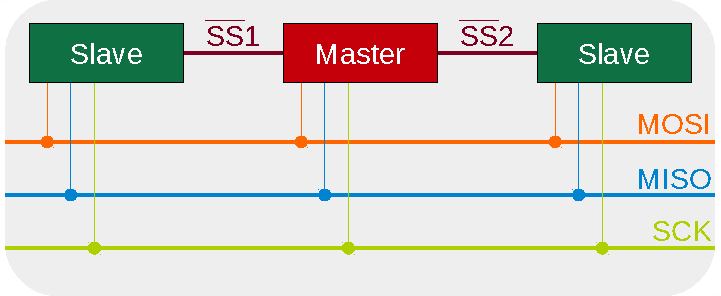
\includegraphics[width=.6\textwidth]{../Presentation/images/spi-bus.pdf}
  \caption{SPI Physical Connection Scheme}
  \label{fig:spi_physical}
\end{figure}

The slave select ($\overline{\text{SS}}$) signal is used by the master node to select the slave it wants to talk to. The serial clock (SCK) signal is again a simple digital clock signal for synchronization. The master-out-slave-in (MOSI) line is used to transmit data from the master to a slave node and the master-in-slave-out (MISO) line is used to transmit data from the slave to the master. This bidirectional transsmission happens simultaneously, so SPI is full-duplex protocol. Figure \ref{fig:spi} shows a timing diagram of the SPI protocol.

\begin{figure}[H]	
	\centering
  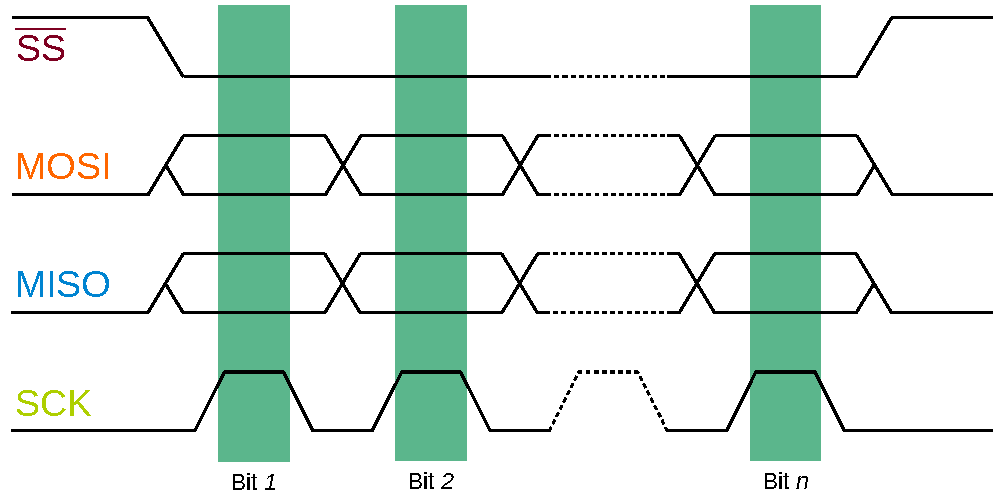
\includegraphics[width=.6\textwidth]{../Presentation/images/spi-timing.pdf}
  \caption{SPI Timing Diagram}
  \label{fig:spi}
\end{figure}

\subsection{Comparison}
Finally I want to compare the two communication protocols with each other. The I2C protocol only needs two signal wires for communication and allows multiple master nodes, this makes it a perfect fit for highly modular applications. However communication is only half-duplex and the communication speed is limited to 5 Mbit/s. In contrast the SPI protocol needs $3 + n$, where $n$ is the amount of slave nodes, and allows only one master on the bus. Therefore SPI is less suited if high modularity is needed. However SPI is full-duplex and offers much higher communication speeds. Therefore SPI is a perfect fit for applications where high communication speed is necessary.

\begin{table}[H]
  \centering
  \begin{tabular}{c|c}
    \textbf{I2C} & \textbf{SPI} \\ \hline
    $2$-wires & $3 + n$ wires \\
    multi-master & single-master \\
    half-duplex & full-duplex \\
    5 Mbit/s & over 10 Mbit/s
  \end{tabular}
  \caption{Comparison Table of I2C and SPI}
  \label{table:i2c_vs_spi}
\end{table}


\nocite{*}
\newpage
\sloppy\printbibliography

\end{document}
